\documentclass[11pt,letterpaper,twocolumn]{article}
\usepackage[utf8]{inputenc}
\usepackage[spanish]{babel}
\usepackage{amsmath}
\usepackage{amsfonts}
\usepackage{amssymb}
\usepackage{float}
\usepackage{graphicx}
\usepackage{subfigure}
\usepackage{listings}
\usepackage[left=2cm,right=2cm,top=2cm,bottom=2cm]{geometry}
\begin{document}
\title{\huge{\textbf{
Simulación de un sistema de N osciladores acoplados con MATLAB\\Simulation of a system of N coupled  oscillators with MATLAB}}}
\author{\small \textit{M. Sabogal $^{1}$}\\
	\small \textit{ $^{1}$ Estudiante del programa de Física, Universidad del Atlántico, Barranquilla-Colombia}}
\date{} 

\twocolumn[
\begin{@twocolumnfalse}
\maketitle
\begin{center}
{\rule[0mm]{160mm}{0.2mm}}
\end{center}
\begin{abstract}
\textit{Se realizo el estudio y análisis del comportamiento de un sistema de 3 y 151 osciladores acoplados, utilizando las herramientas computacionales de MATLAB, corroborando algunas de las características dinámicas que presentan estos sistemas, como su periodicidad, un atractor global en el espacio de fases y la conservación de la energía total del sistema. De igual manera se simulo 100 veces el caso de 101 osciladores acoplados de masas iguales y con valores aleatorios de las constantes de elasticidad de los resortes, en tres diferentes intervalos de desorden, $(0$.$9,1$.$1)$, $(0$.$8,1$.$2)$ y $(0$.$7,1$.$3)$ respectivamente, con el fin de determinar valores estadísticos que proveen información acerca de la manera cómo el ancho de desorden, dificulta el transporte de la energía de la perturbación inicial central hacia los extremos.\\
\\
\textbf{Palabras claves: Oscilador, acoplado, perturbación, simulación.}}
\begin{center}
\textbf{Abstract} 
\end{center}
\par 
\textit{it was carried out the study and analysis of the behavior of a system of 3 and 151 coupled oscillators , using the MATLAB computational tools, verifying some of the dynamic characteristics that these systems present, such as their periodicity, a global attraction in the phase space, and the conservation of the total energy of the system. Likewise, the case of 101 coupled oscillators of equal masses and with random values of elasticity constants of the springs, in the different intervals, $ (0 $. $ 9,1 $. $ 1) $ , $ (0 $. $ 8,1 $. $ 2) $ and $ (0 $. $ 7,1 $. $ 3) $ respectively, was simulated 100 times, in order to determine the statistical values that provied information about the way the width of disorder makes it difficult to transport the energy from the initial central disturbance to the extremes.\\
\\
\textbf{Keywords: Oscillators, coupled, disturbance, simulation.}}
\end{abstract}
\begin{center}
{\rule[0mm]{160mm}{0.2mm}}
\end{center}
\end{@twocolumnfalse}
]

\section*{\normalsize{INTRODUCCIÓN}} 
El oscilador armónico es uno de los sistemas más estudiados en la física, ya que al observar la naturaleza nos damos cuenta de que muchos procesos físicos son repetitivos, es decir presentan un comportamiento cíclico. Una masa sujeta al extremo de un péndulo o de un resorte, la carga eléctrica almacenada en un condensador, las cuerdas de un instrumento musical, y las moléculas de una red cristalina son ejemplos de sistemas físicos que a menudo realizan un movimiento oscilatorio.\\ 
\par
Un sistema formado por dos osciladores iguales tipo masa-resorte “conectados”, se denomina un sistema de osciladores acoplado, determinados movimientos colectivos del sistema, se comportan como simples osciladores armónicos, sin embargo, a medida que aumenta el numero de osciladores, la diferencia entre sus masas, y la de sus constantes de acoplamiento, la complejidad del movimiento colectivo de estos aumenta, haciendo de estos, sistemas ricos de estudio y bases para el modelamiento de sistemas mas complejos. Estos sistemas mecánicos de muchas partículas, donde cada una de ellas oscila alrededor de su posición de equilibrio ( vibra ), han servido conceptualmente a la física para modelar el comportamiento mecánico, térmico y magnético de los sólidos, contribuyendo así con el desarrollo de la mecánica estadística y la termodinámica$^{[1]}$. Se desea estudiar con énfasis el sistema de tres osciladores acoplados, y el de N=101 osciladores unidimensionalmente, a partir de simulaciones computacionales en MATLAB. 
\subsection*{Sistema de tres oscialdores acoplados}
En primera instancia con el fin de estudiar un sistema formado por tres osciladores acoplados, se tomo como modelo el sistema formado por tres partículas de masas $m_{1},m_{2},m_{3}$ situadas en los extremos de 4 resortes de constante elástica diferentes, como se observa en la figura. El acoplamiento unidimensional se efectúa uniendo las partículas mediante los muelle, y considerando que los resortes de los extremos están atados a paredes inamovibles$^{[2]}$.
\begin{figure}[h!]
\begin{center}
\includegraphics[scale=0.4]{3-o.jpeg}
\end{center}
\end{figure}

\par 
Teniendo en cuenta que el sistema presenta ausencia de fuerzas disipativas y externas, a excepción de la perturbaron inicial, por el principio de la conservación de la energía, se tiene que la energía total del sistema es una constante de la forma:
$$E_{t}=K+U$$
\par 
Donde $K$ representa la energía cinética del sistema y $U$ la potencial elástica. 
$$K=\sum_{i=1}^{3} \dfrac{1}{2} m_{i} \dot{x}_{i}^{2}$$ 
$$U=\dfrac{1}{2}k_{1}x_{1}^{2} +  \dfrac{1}{2}k_{2}(x_{2}-x_{1})^{2} + \dfrac{1}{2}k_{3}(x_{3}-x_{2})^{2} + \dfrac{1}{2}k_{4}x_{3}^{2}$$
\par 
Recordando que para sistemas conservativos se tiene:
$$\vec{F_{i}}=- \vec{\nabla}U_{i}=-(\dfrac{\partial U_{i}}{\partial x_{i}},0,0)$$ 
\par 
A partir de la segunda ley de newton y considerando que la partículas solo interactúa con sus vecinas de manera unidimensional, en ausencia de un campo gravitacional externo, se deduce las expresiones para describir el movimiento de cada partícula:
$$\ddot{x_{1}}=-\dfrac{(k_{1}+k_{2})}{m_{1}}x_{1} + \dfrac{k_{2}}{m_{1}}x_{2}$$
\begin{equation}
\ddot{x_{2}}=-\dfrac{(k_{2}+k_{3})}{m_{2}}x_{2} + \dfrac{k_{2}}{m_{2}}x_{1} + \dfrac{k_{3}}{m_{2}}x_{3}
\label{conjunto}
\end{equation}
$$\ddot{x_{3}}=-\dfrac{(k_{3}+k_{4})}{m_{3}}x_{3} + \dfrac{k_{3}}{m_{3}}x_{2}$$
\par 
La ecuaciones de \ref{conjunto} son el conjunto de EDO de segundo orden acopladas que se debe resolver para tener pleno entendimiento del fenómeno, teniendo en consideración que en este caso las aceleraciones no depende explícitamente del tiempo sino de la posición de la partícula con respecto al a sus vecinas y del valor de las constantes elásticas de los resortes que las acoplan.\\
\par 
Reescribiendo el sistema de ecuaciones diferenciales anterior \ref{conjunto}, se tiene: 
\[
\dfrac{d^{2}}{dt^{2}} \left(
\begin{matrix}
x_{1}\\
x_{2}\\
x_{3}
\end{matrix} \right) = \hat{M_{3}}  \left(
\begin{matrix}
x_{1}\\
x_{2}\\
x_{3}
\end{matrix} \right)
\] 
\par 
Donde $\hat{M}$, es la matriz de frecuencias al cuadrado del sistema: 
\[ \hat{M_{3}} = \left[
\begin{matrix}
-\dfrac{(k_{1}+k_{2})}{m_{1}} & \dfrac{k_{2}}{m_{1}} &  0 \\
\\
 \dfrac{k_{2}}{m_{2}} & -\dfrac{(k_{2}+k_{3})}{m_{2}} & \dfrac{k_{3}}{m_{2}}\\
\\
 0 &  \dfrac{k_{3}}{m_{3}} & -\dfrac{(k_{3}+k_{4})}{m_{3}}
\end{matrix} \right]
\]
Con la intención de resolver el sistema de manera computacional, se plantea pasar del sistema de tres EDO de segundo orden a un sistema de seis EDO de primer orden, realizando las sustituciones $p_{i}=x_{i}$ y $q_{i}=\dfrac{dx_{i}}{dt}$, obteniendo el sistema de ecuaciones equivalente a resolver, de la forma: 
\[
\dfrac{d}{dt} \left(
\begin{matrix}
p_{1}\\
p_{2}\\
p_{3}\\
q_{1}\\
q_{2}\\
q_{3}
\end{matrix} \right) = \hat{M1}  \left(
\begin{matrix}
p_{1}\\
p_{2}\\
p_{3}\\
q_{1}\\
q_{2}\\
q_{3}
\end{matrix} \right)
\] 
\par 
Donde $\hat{M1}$ presentan la siguiente forma, siendo $\hat{0}$ una matriz $3$x$3$ de ceros y $I_{3}$ la matriz identidad de orden $3$: 
\[ \hat{M1} = \left[
\begin{matrix}
\hat{0} &  I_{3}\\
\hat{M_{3}} & \hat{0}
\end{matrix}  \right]
\]
\subsection*{Sistema de N oscialdores acoplados}
Tomando cómo base el modelamiento de tres osciladores acoplados, este se generalizo para N de estos osciladores, encontrando a partir de la energía potencial del sistema, el conjunto de N EDO acopladas de segundo grado que describen la evolución del sistema: 
\[
\dfrac{d^{2}}{dt^{2}} \left(
\begin{matrix}
x_{1}\\
x_{2}\\
x_{3}\\
\vdots\\
x_{n}
\end{matrix} \right) = \hat{M_{n}}  \left(
\begin{matrix}
x_{1}\\
x_{2}\\
x_{3}\\
\vdots\\
x_{n}
\end{matrix} \right)
\] 
Donde $\hat{M_{n}}$ presenta la forma: 
{\fontsize{5.5}{15}\selectfont
\[\left[
\begin{matrix}
-\dfrac{(k_{1}+k_{2})}{m_{1}}&\dfrac{k_{2}}{m_{1}}&0&\dots&0 & 0 \\
\\
\dfrac{k_{2}}{m_{2}}&-\dfrac{(k_{2}+k_{3})}{m_{2}}&\dfrac{k_{3}}{m_{2}}&\dots&0&0\\
\\
0 &\dfrac{k_{3}}{m_{3}}&-\dfrac{(k_{3}+k_{4})}{m_{3}}&\dots&0&0\\
\vdots&\vdots&\vdots&\dots&\vdots&\vdots\\
\vdots&\vdots&\vdots&\dots&\vdots&\vdots\\
 0 & 0 & 0 & \dots & \dfrac{k_{n+1}}{m_{n}} &-\dfrac{(k_{n}+k_{n+1})}{m_{n}}
\end{matrix} \right]
\]}
\par 
De igual manera al caso de tres osciladores, se realizan las sustituciones pertinentes, con el fin de encontrar el sistema de ecuaciones equivalentes de primer grado, obteiendo: 
\[
\dfrac{d}{dt} \left(
\begin{matrix}
p_{1}\\
p_{2}\\
p_{3}\\
\vdots\\
p_{n}\\
q_{1}\\
q_{2}\\
q_{3}\\
\vdots\\
q_{n}
\end{matrix} \right) = \hat{M1}  \left(
\begin{matrix}
p_{1}\\
p_{2}\\
p_{3}\\
\vdots\\
p_{n}\\
q_{1}\\
q_{2}\\
q_{3}\\
\vdots\\
q_{n}
\end{matrix} \right)
\] 
\par 
Donde $\hat{M1}$ presentan la siguiente forma, siendo $\hat{0}$ una matriz $n$x$n$ de ceros y $I_{n}$ la matriz identidad de orden $n$, es decir, ésta es una matriz cuadrada $2n$x$2n$: 
\[ \hat{M1} = \left[
\begin{matrix}
\hat{0} &  I_{n}\\
\hat{M_{n}} & \hat{0}
\end{matrix}  \right]
\]
\subsection*{Grado de participacion y propagación de la energia}
Con el fin de observar la distribución espacial de varias soluciones, en nuestro caso de los N osciladores, se usa una útil cantidad, llamada grado de participación, definida de la siguiente forma, donde $E_{t_{i}}$ es la energía total individual del oscilador i-esimo: 
\begin{equation}
R_{E}(t)=\dfrac{\left( \sum_{i=1}^{N}\lvert E_{t_{i}}(t) \rvert^{2} \right)^{2}}{\sum_{i=1}^{N}\lvert E_{t_{i}}(t) \rvert^{4}} 
\end{equation}
\par 
La cual suministra la información de cuantos sitios son excitados en la propagación de la perturbación inicial, teniendo un máximo cuando $R_{E}=N$ es decir todos los osciladores están aportando de manera activa al movimiento$^{[3]}$. A partir de la perturbación inicial, las energías de cada oscilador dependerá directamente de las distancias entre sus vecinas, es decir de la amplitud relativa de su movimiento, sin embargo es posible que su amplitud relativa sea muy pequeña y que esta presente en mayor grado energía cinética, con la intención de comparar la premisa anterior, se plantea una segunda cantidad que representa el grado de participación en función de las amplitudes de los osciladores ($A_{i}$), de la forma: 
\begin{equation}
R_{A}(t)=\dfrac{\left( \sum_{i=1}^{N}\lvert A_{i}(t) \rvert^{2} \right)^{2}}{\sum_{i=1}^{N}\lvert A_{i}(t) \rvert^{4}} 
\end{equation}
\par 
Al perturbar el sistema propuesto, justo en la mitad, se desencadena una propagación o transporte de la energía hacia los extremos, con el fin de medir la difusión de esta energía, es decir la rapidez con la que se propaga la energía, se utilizará el desplazamiento cuadrático medio$^{[3]}$, definido en nuestro caso como: 
\begin{equation}
m_{2}=\dfrac{\sum_{i=1}^{N} i^{2} \lvert E_{t_{i}} \rvert^{2} }{\sum_{i=1}^{N} \lvert E_{t_{i}} \rvert^{2}}
\end{equation}
\par 
Sin embargo, cómo en el modelo de estudio las masas de las partículas y las constantes de los resortes pueden ser diferentes, la energía puede que no se reparta de manera simétrica con respecto al centro, si este se perturba. En aras de comprobar esto, se utilizara una cantidad denotada como la media ponderada de la energía de los osciladores: 
\begin{equation}
m_{1}=\dfrac{\sum_{i=1}^{N} i \lvert E_{t_{i}} \rvert^{2} }{\sum_{i=1}^{N} \lvert E_{t_{i}} \rvert^{2}}
\end{equation}

\section*{-Implementación, interpretación física y resultados}
Con el fin de estudiar el comportamiento de un sistema de osciladores acoplados y sus características, se realizaron diferentes simulaciones del modelo, para $N=3$ osciladores y $N=101$ mediante las herramientas computacionales de MATLAB.\\
\par 
En primera instancia se estableció el numero $N$ de osciladores acoplados, el intervalo de tiempo de estudio, y las condiciones dinámicas iniciales del sistema $(x_{o},v_{o})=(p_{o},q_{o})$; en el presente análisis solo se perturbo el oscilador en la posición del medio, mientras los demás se encontraban inmóviles, es decir la posición inicial del oscilador en el medio es 1, mientras la de los demás $N-1$ restantes son cero, y todas las velocidades iniciales son cero, esto se logro utilizando la función \textit{zeros()} de MATLAB, luego se asignaron los valores de las masas y constantes elásticas del sistema, de manera aleatoria entre los intervalos $(m_{i},m_{f})$ y $(k_{i},k_{f})$ respectivamente, mediante la función \textit{rand()}.\\ 
\par 
Posteriormente con los valores de las masas y constantes elásticas, se determinaron los diagonales de la matriz $\hat{M_{n}}$ mencionada anteriormente, y nuevamente mediante la función \textit{zeros()} y la función \textit{eye()} se determinaron las matrices de ceros y la matriz identidad de orden N, de la matriz $\hat{M1}$ de la ecuación 3. Finalmente utilizando el Runge kutta de cuarto orden de MATLAB mediante la función \textit{ode45()}, fue posible calcular cada una de las posiciones y velocidades de los osciladores acoplados después de un tiempo $t_{f}$ transcurrido desde la perturbación inicial.
\begin{figure}[h!]
\begin{center}
\subfigure[] {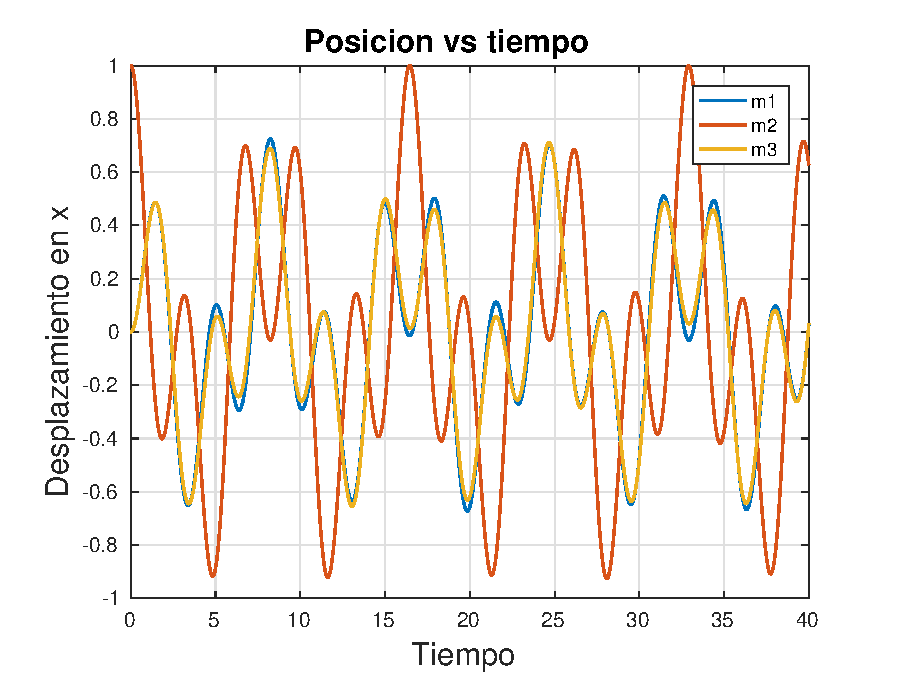
\includegraphics[scale=0.6]{pos.eps}}
\subfigure[] {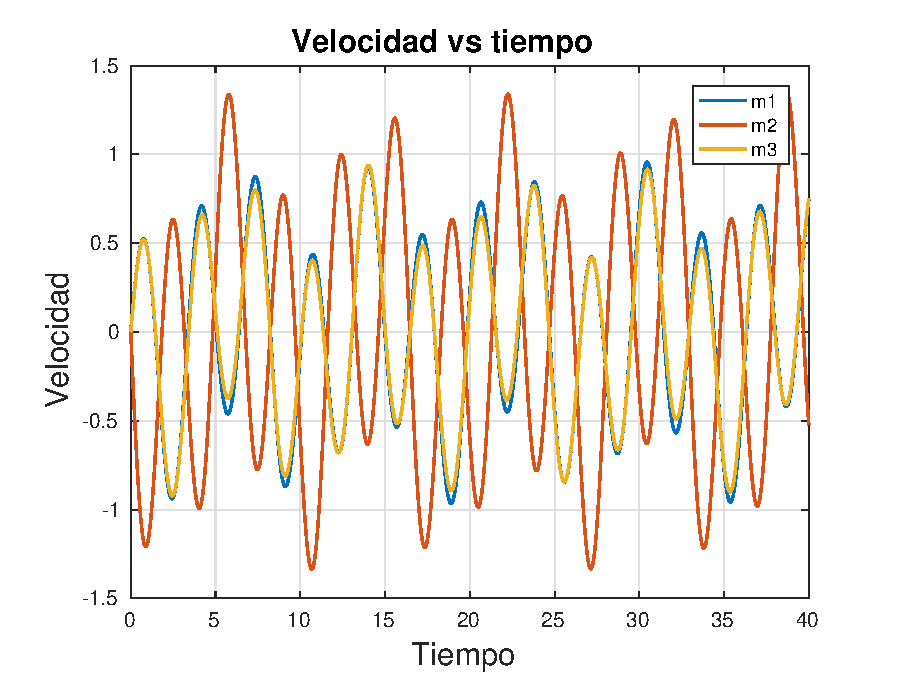
\includegraphics[scale=0.6]{vel.eps}}
\caption{Sistema de 3 osciladores acoplados con $k_{1}=1.0087$, $k_{2}=1.0903$, $k_{3}=1.0706$ , $k_{4}=0.9620$ y masas iguales. (a) Posiciones en funcion del tiempo. (b) velocidades en funcion del tiempo.}
\end{center}
\label{pos}
\end{figure}
\par 
En la figura $1$ se visualiza el desplazamiento en x y la velocidad en función del tiempo, para tres osciladores acoplados ($N=3$) de masa diferentes y constantes diferentes, en la que se puede apreciar el comportamiento periódico que estas presentan, y como el movimiento de cada partícula se ve afectado por el de sus vecinas$^{[4]}$, de igual manera se observa como la velocidad de cada oscilador se ve afectada por la distancia relativa a sus vecinas.\\
\par 
Ya que las fuerzas involucradas son conservativas, la energía del sistema se debe conservar, cómo se observa en la figura $2$ (a), la cual presenta las energías cinéticas (K) y potencial (U) en función del tiempo, y la energía total del sistema, la cual es una constante; de manera similar en la figura $2$ (b) se percibe como evoluciona la energía de cada oscilador en el tiempo.\\
\begin{figure}[h!]
\begin{center}
\subfigure[] {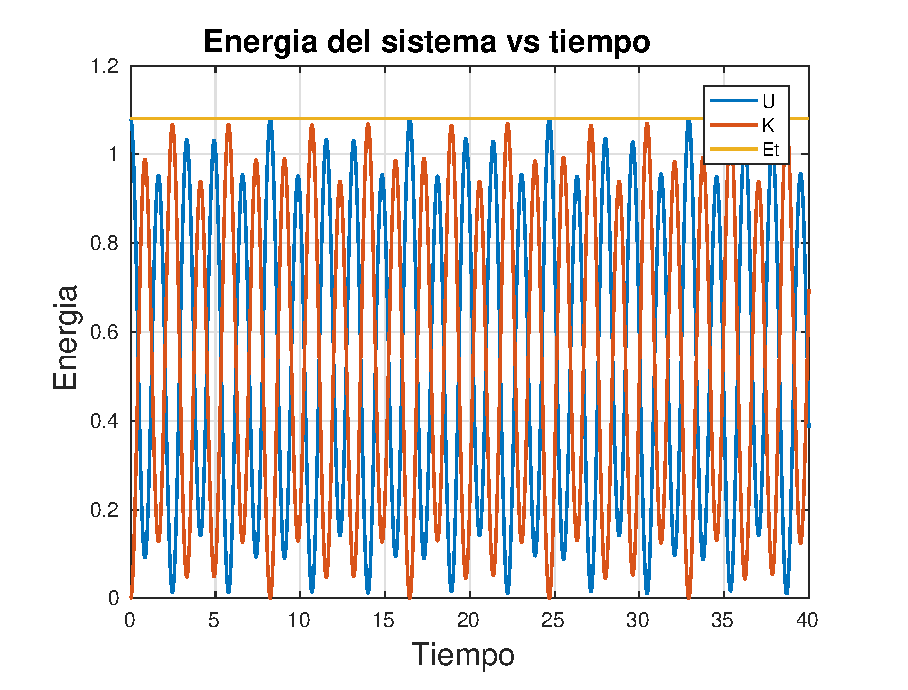
\includegraphics[scale=0.65]{ene.eps}}
\subfigure[] {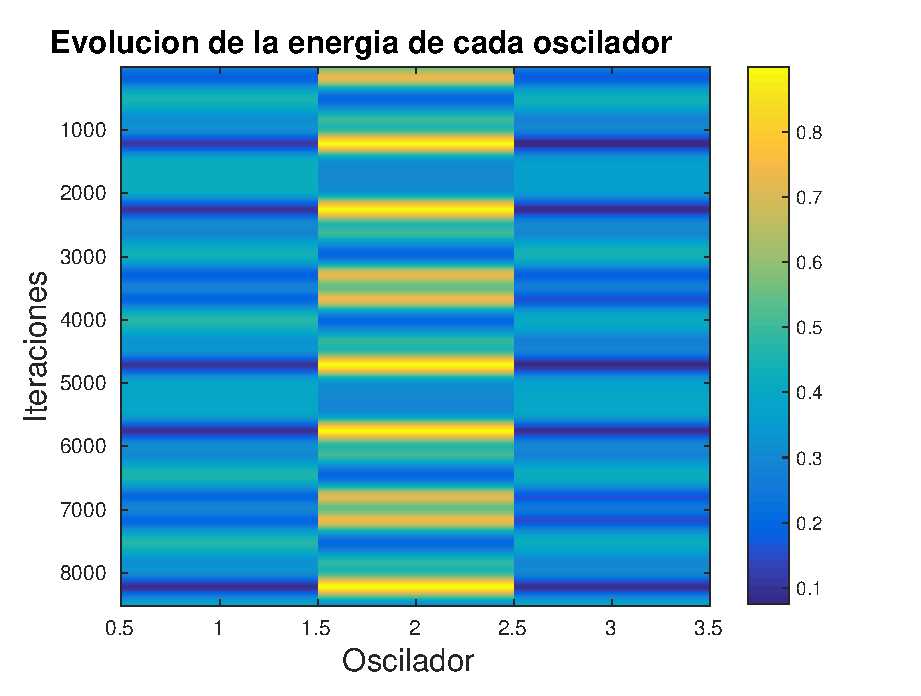
\includegraphics[scale=0.65]{energia.eps}}
\caption{Sistema de 3 osciladores acoplados con $k_{1}=1.0087$, $k_{2}=1.0903$, $k_{3}=1.0706$ , $k_{4}=0.9620$ y masas iguales. (a) Energias del sistema en funcion del tiempo. (b) Energia de cada oscilador en el tiempo.}
\end{center}
\label{ene}
\end{figure}
\par 
Del análisis anterior se observa que el modelo es consistente para $N=3$ osciladores, con la intención de verificar si el modelo implementado es consistente para N muy grades, se realizo una simulación de $N=151$ osciladores. Comprobando como se aprecia en la figura $3$, que el modelo es consistente para N pequeñas o muy grandes, ya que la energía total del sistema se conserva (b), y estas presentan movimientos acoplados (a) entre si. \\
\begin{figure}[h!]
\begin{center}
\subfigure[] {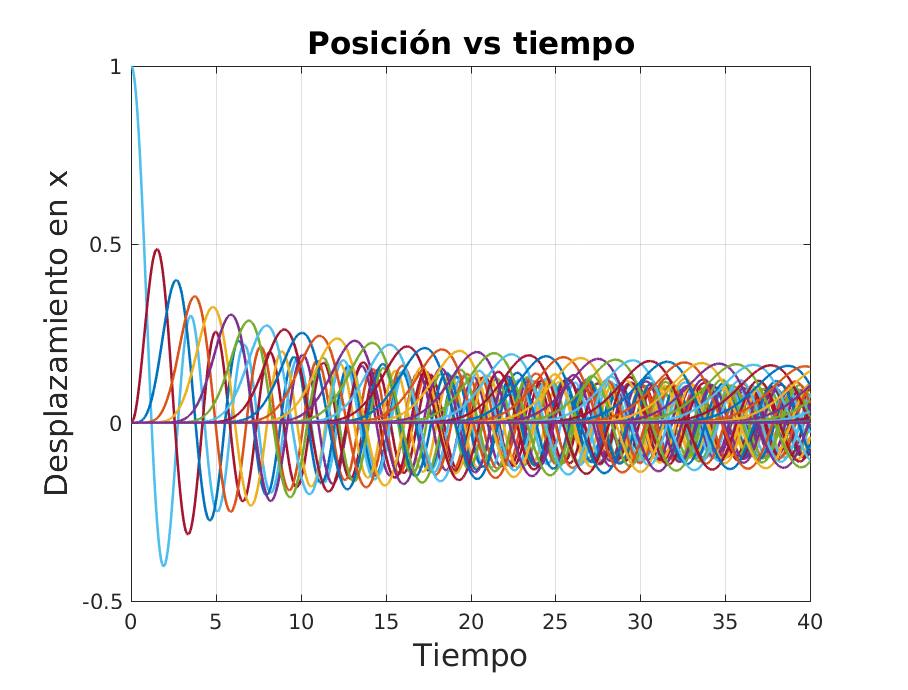
\includegraphics[scale=0.67]{151.eps}}
\subfigure[] {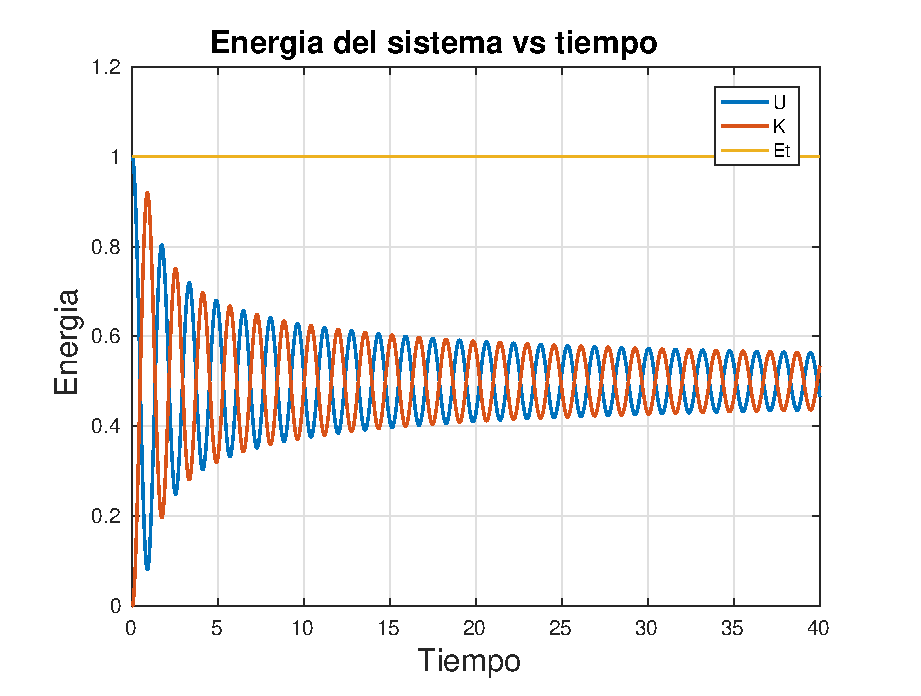
\includegraphics[scale=0.67]{e151.eps}}
\caption{Sistema de 151 osciladores acoplados con constantes elasticas y masas iguales. (a) Posiciones en funcion del tiempo. (b) Energia del sistema en funcion del tiempo.}
\end{center}
\end{figure}
\par 
De la gráfica anterior, se puede visualizar que las energías del sistema se comportan como las de un solo oscilador, figura $3$ (b), oscilando alrededor de su punto de equilibrio, lo cual sugiere, que en el diagrama de fases del sistema existe un atractor global como se observa en la figura $4$ (a), y al graficar las posiciones del sistema para cada instante utilizando la función \textit{imagesc()}, se aprecia en la figura $4$ (b), como evoluciona la posición de cada oscilador, percibiendo que estas varían principalmente entre $0.5$ y $-0.5$, a excepción de la perturbación inicial. Con la intención de dilucidar la propagación de la perturbación, se obtuvieron los valores absolutos de las posiciones utilizando la función \textit{abs()}, y nuevamente utilizando la función \textit{imagesc()} se graficaron éstos valores, donde observa en la figura $4$ (c), como se propaga la perturbación central hacia los extremos.\\
\begin{figure}[h!]
\begin{center}
\subfigure[] {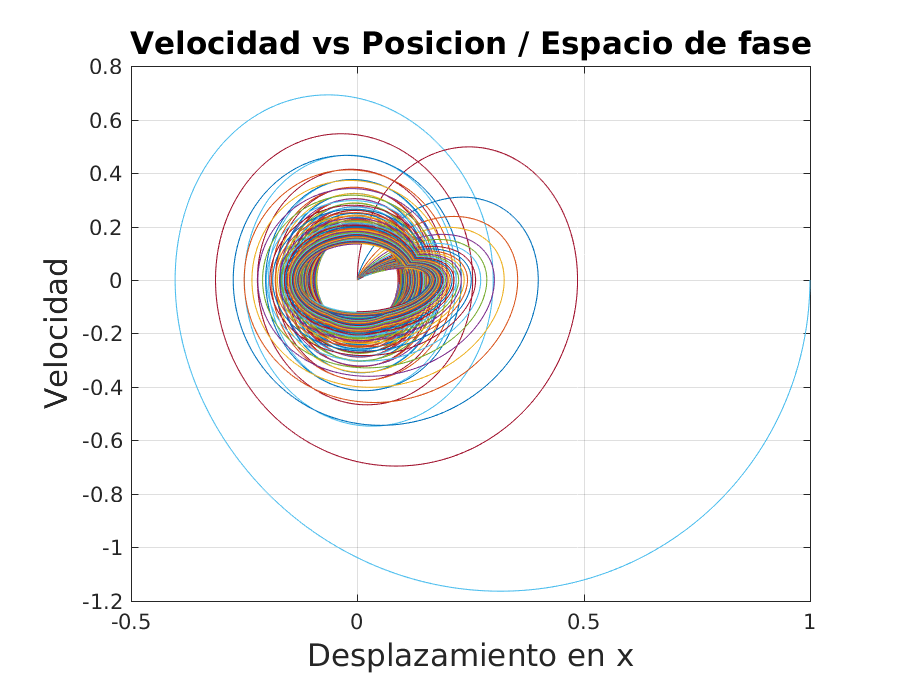
\includegraphics[scale=0.56]{espaciof.eps}}
\subfigure[] {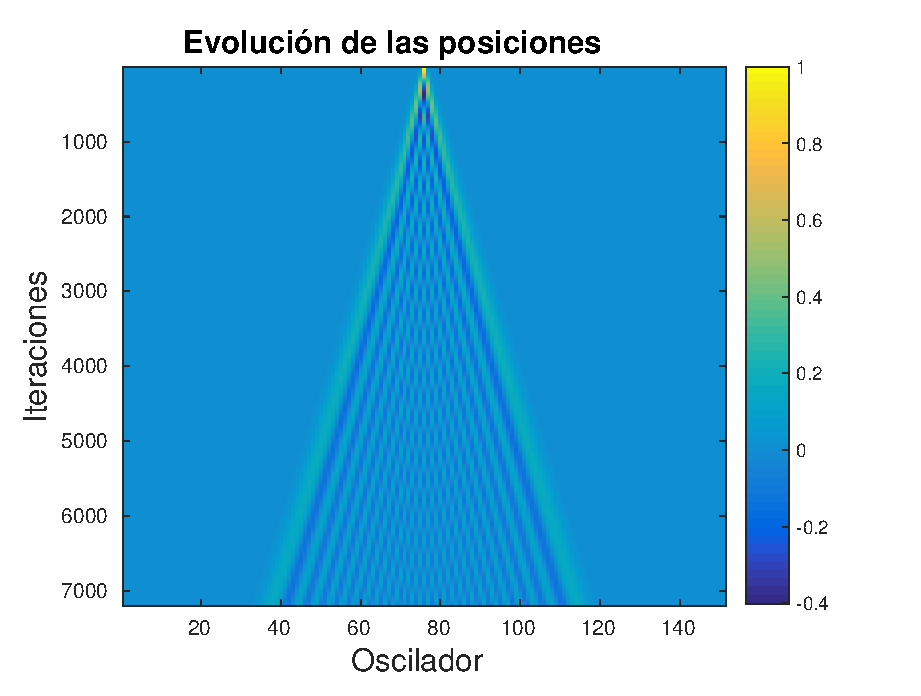
\includegraphics[scale=0.56]{per.eps}}
\subfigure[] {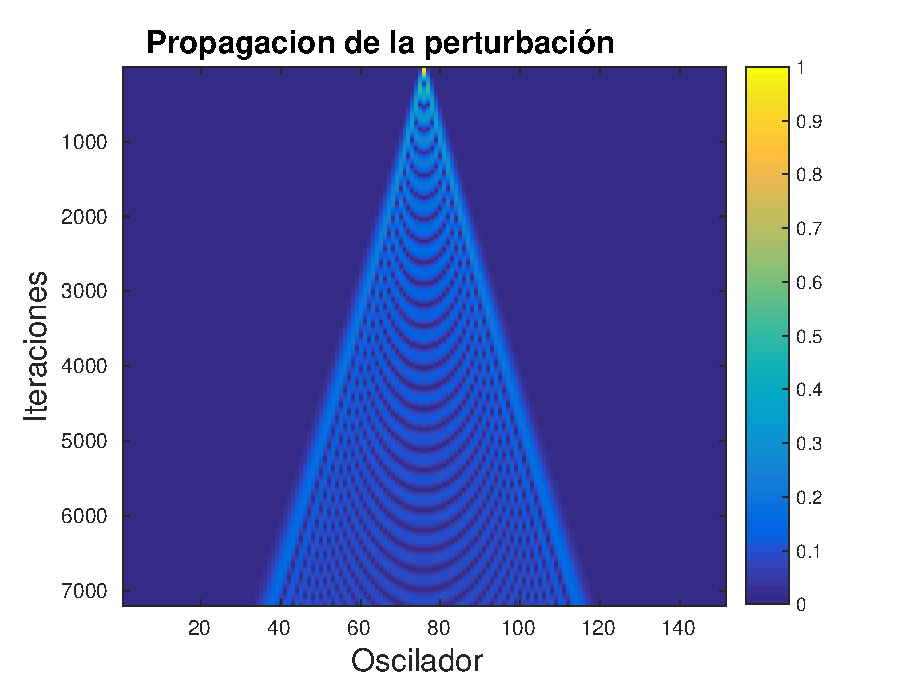
\includegraphics[scale=0.56]{abper.eps}}
\caption{Sistema de la figura $3$ (a) Espacio de fase del sistema (b) Evolucion de las posiciones en el tiempo (c) Propagación de la perturbación.}
\end{center}
\end{figure}
\par 
De la ultima gráfica de la figura $4$, se observa que la propagación de la perturbación central excita a los osciladores desde el centro hacia los extremos; con el fin de visualizar numéricamente como la propagación de la perturbación afecta el estado de los osciladores en función del tiempo, se calculo el grado de participación promedio tanto de la ecuación $2$ y de la ecuación $3$, como se observa en la figura $5$ (a) para 100 simulaciones de $N=101$ osciladores con masas iguales y constantes elásticas aleatorias en un intervalo ($k_{i}$,$k_{f}$).\\
\begin{figure}[h!]
\begin{center}
\subfigure[] {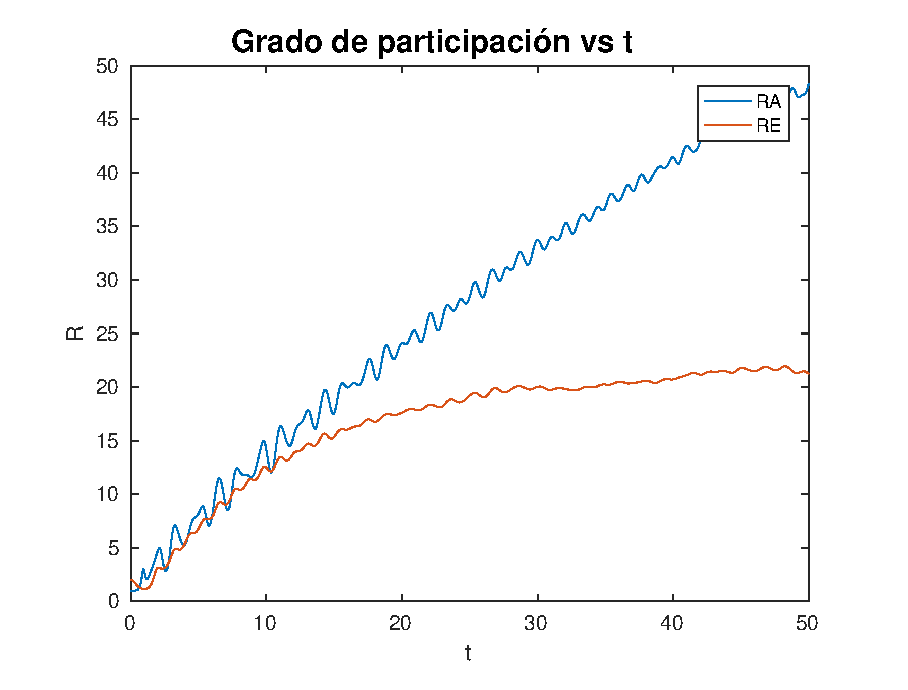
\includegraphics[scale=0.55]{R.eps}}
\subfigure[] {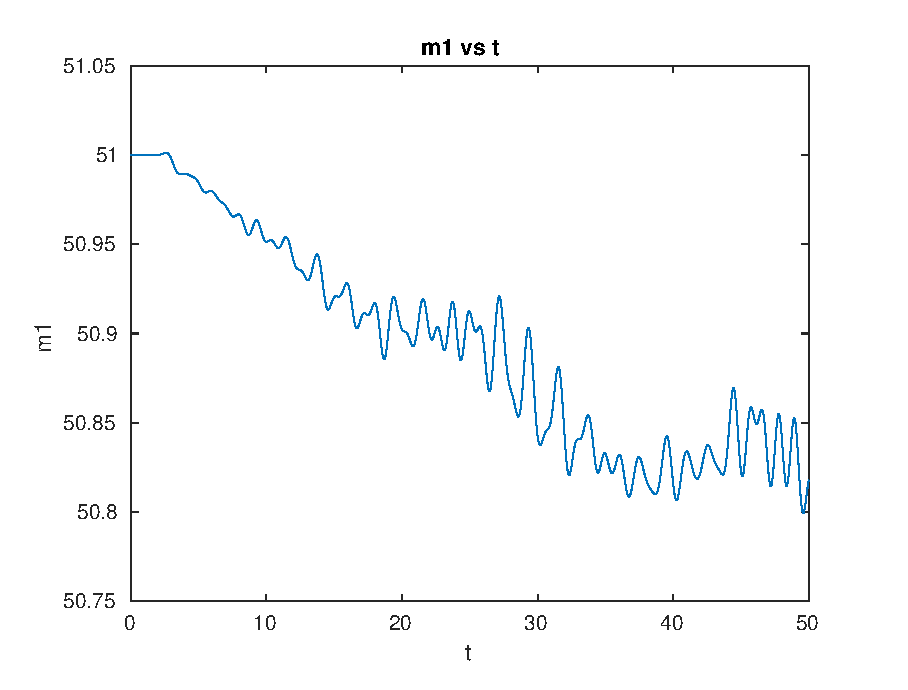
\includegraphics[scale=0.55]{m1-l.eps}}
\subfigure[] {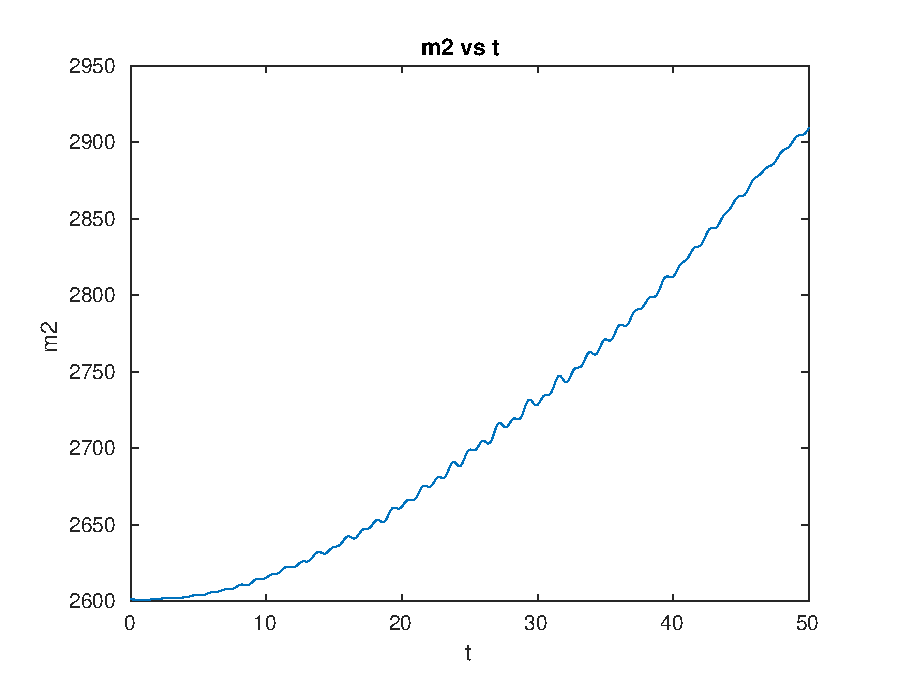
\includegraphics[scale=0.55]{m2.eps}}
\caption{Sistema de 101 oscialdores acoplados, de masas iguales y valores aleatorios de las constantes de elasticidad en intervalo de $(0$.$9,1$.$1)$. (a) Grado de participacion (b) $m1$ (c) $m2$ en funcion del tiempo.}
\end{center}
\end{figure}
\par 
Esto se realizo tomando en consideración que la energía total individual de cada oscilador es la suma de su energía cinética y la energía potencial elástica, donde ésta, para los acoplados es la mitad de la energía elástica del resorte, debido a que debe repartirse entre los dos osciladores acoplados por el resorte. Observando una diferencia notable entre ellas cómo se hipotizo previamente. A partir de estas energías, también fue posible determinar la media ponderada (a) de la energía al cuadrado del sistema y la desviación cuadrática media (b) para el caso anterior, como se observa en la figura $5$.\\
\par 
Con el fin de apreciar como el ancho de desorden afecta el grado de participación y la manera como se transporta la energía en un sistema de N osciladores acoplados, con valores aleatorios de las constantes de elasticidad, se calcularon los grados de participación promedio, media ponderada y sus desplazamiento cuadrático medio, como se observa en la figuras $5,6$ y $7$, para 100 simulaciones de $N=101$ osciladores con masas iguales y constantes elásticas aleatorias en dos diferentes intervalos de aleatoriedad ($k_{i}$,$k_{f}$).\\
\begin{figure}[h!]
\begin{center}
\subfigure[] {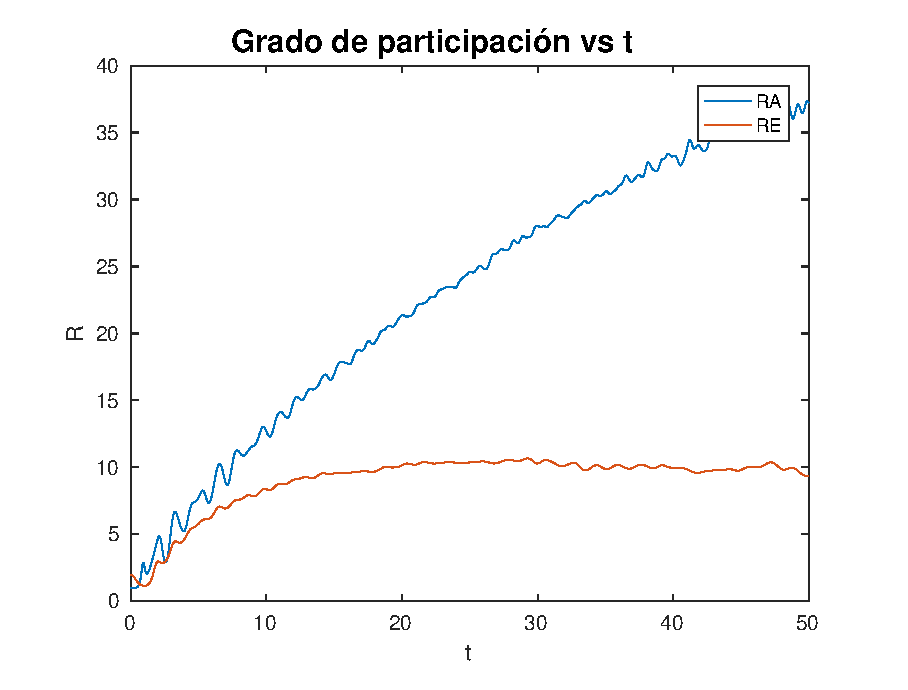
\includegraphics[scale=0.55]{R2.eps}}
\subfigure[] {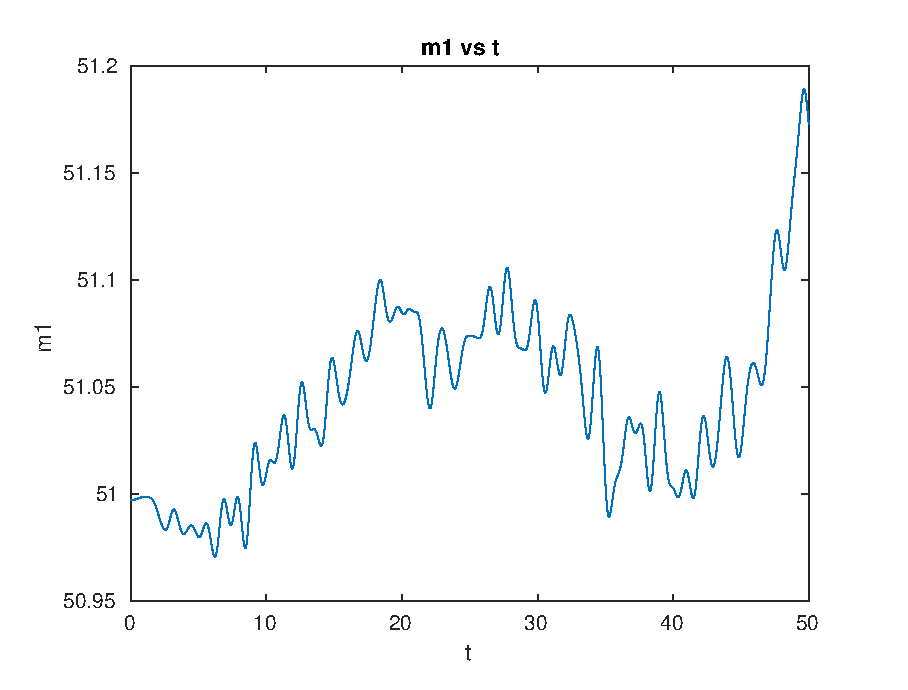
\includegraphics[scale=0.55]{m12.eps}}
\subfigure[] {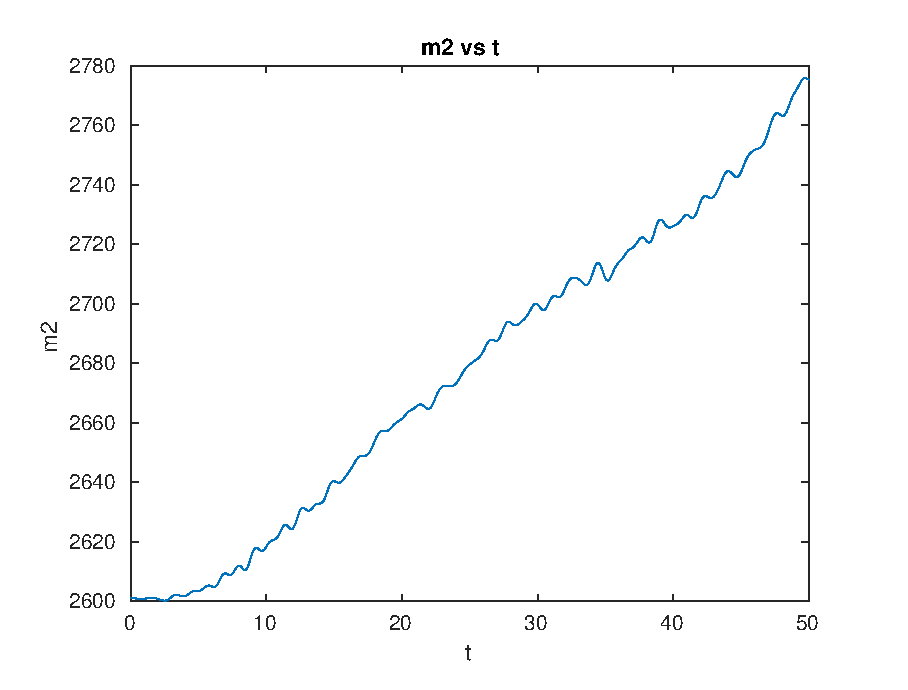
\includegraphics[scale=0.55]{m22.eps}}
\caption{Sistema de 101 oscialdores acoplados, de masas iguales y valores aleatorios de las constantes de elasticidad en intervalo de $(0$.$8,1$.$2)$. (a) Grado de participacion (b) $m1$ (c) $m2$ en funcion del tiempo.}
\end{center}
\end{figure}

\begin{figure}[h!]
\begin{center}
\subfigure[] {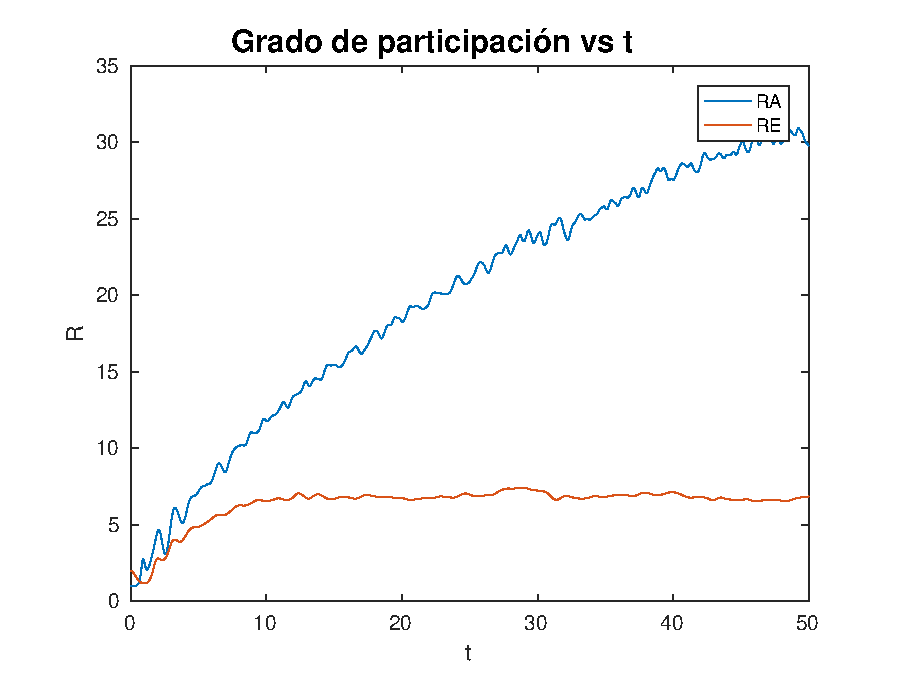
\includegraphics[scale=0.55]{R3.eps}}
\subfigure[] {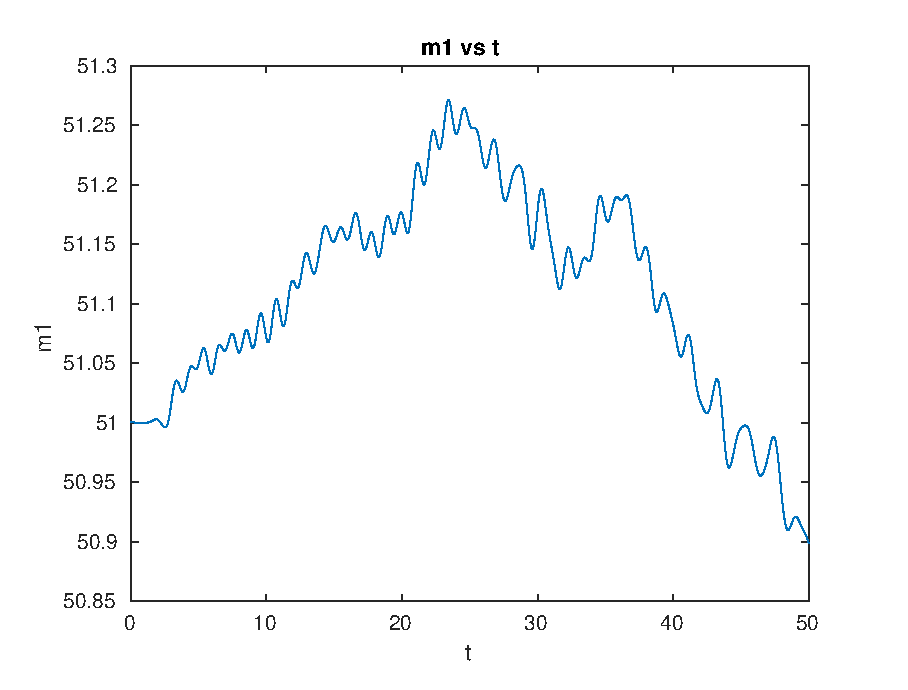
\includegraphics[scale=0.55]{m13.eps}}
\subfigure[] {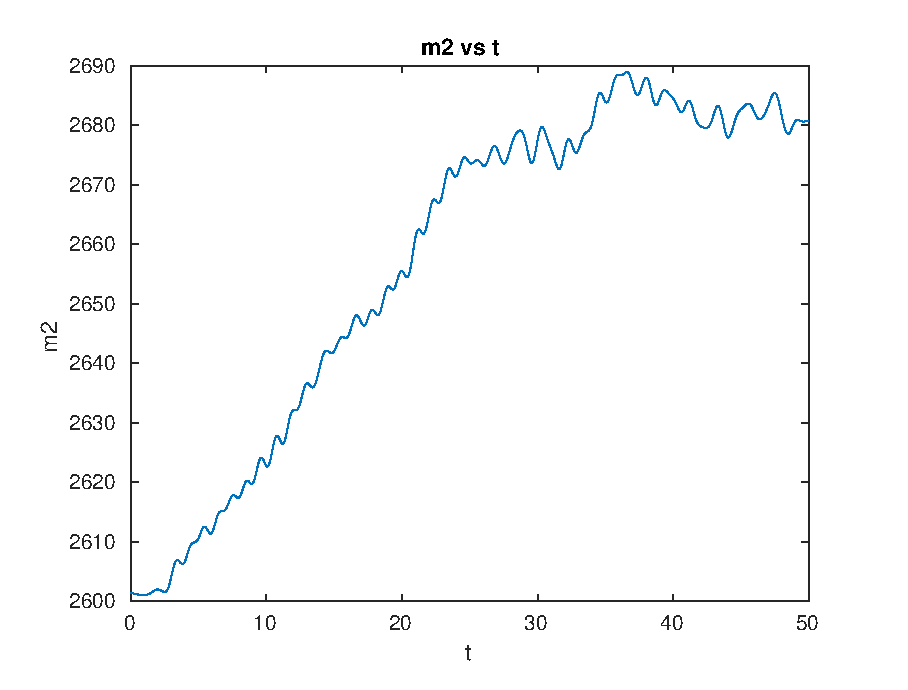
\includegraphics[scale=0.55]{m23.eps}}
\caption{Sistema de 101 oscialdores acoplados, de masas iguales y valores aleatorios de las constantes de elasticidad en intervalo de $(0$.$7,1$.$3)$. (a) Grado de participacion (b) $m1$ (c) $m2$ en funcion del tiempo.}
\end{center}
\end{figure}
\par 
Con respecto a los grados de participación en función del tiempo, se aprecia como disminuyen a medida que aumenta el ancho de desorden, debido a que existe una posible mayor diferencia entre los valores de las constantes que acoplan a dos masas vecinas, provocando un aumento en la dificultan para transportar la energía del centro hacia los extremos, como se aprecia en las figuras de $m2$, de las figuras de $m1$ se visualiza como oscilan alrededor del punto central y a medida que aumenta el ancho, la amplitud de éstas oscilaciones aumentan. 
\section*{\normalsize{CONCLUSIÓN}}
Mediante las herramientas computacionales de MATLAB, se pudo estudiar y analizar el comportamiento de un sistema de 3 y 151 osciladores acoplados, comprobando que ambos presentan un comportamiento periódico, que el desplazamiento o amplitud de una partícula se ve influenciado por el de sus vecinas, la velocidad de cada oscilador se ve afectada por la distancia relativa con respecto a sus vecinas, la energía total del sistema se conserva, que ambas presentan un atractor global en el espacio de fases, también se observo como se propaga la perturbación inicial central hacia los extremos. Posteriormente se simulo 100 veces el caso de 101 osciladores acoplados de masas iguales y con valores aleatorios de las constantes de elasticidad de los resortes, en tres diferentes intervalos de desorden, $(0$.$9,1$.$1)$, $(0$.$8,1$.$2)$ y $(0$.$7,1$.$3)$ respectivamente, encontrando que a medida que aumenta el ancho de desorden en el valor de las constantes elásticas, el grado de participación disminuye, los valores de $m1$ oscilan con mayor amplitud con respecto al punto central y de igual forma que el desplazamiento cuadrático medio disminuye. En conclusión se observa que a medida que aumenta el ancho de desorden, es mas difícil repartir la energía inicial de la perturbaron central hacia los extremos.  
\section*{Referencias} 
\begin{itemize} 
\item[[ 1]] Miguel Nebot. Oscilaciones acopladas. Departamento de Física Teórica – IFIC. Universidad de Valencia. 
\item[[ 2]] Edson Plasencia Sánchez. Simulación de un sistema de múltiples osciladores acoplados unidimensionales. Universidad Nacional de Ingeniería. Lima perú-2009.

\item[[ 3]] Cristian Mejía Cortés, Mario I. Molina. Interplay of disorder and PT symmetry in one-dimensional optical lattices. Phys. Rev. A 91, 033815 (2015). 

\item[[ 4]] Sergio Velásquez, Ronny Velásquez. Revista Interdisciplinar de Estudios en Ciencias Básicas e Ingenierías.
Año 2014, Julio-Diciembre, Vol. (1) N$^{\circ}$(2) ISSN 2389-9484.
\end{itemize}
\subsection*{Anexos}

\begin{lstlisting}
1. Codigo en MATLAB para
la simulacion de 3 y 151
ociladores acoplados. 

% Condiciones de entrada
N=101; tf=50; 

% Condiciones iniciales
x0=zeros(N,1); x0(floor(N/2)+1)=1;
v0=zeros(N,1); X0=[x0;v0]; 

% Asignacion de parametros extremos
ki= 0.9; kf= 1.1; mi=1; 
mf=1; iden=eye(N); cero=zeros(N); 

% Asigacion de parametros
mm= mi + (mf-mi)*rand(1,N); 
kk= ki + (kf-ki)*rand(1,N+1); 

% Diagonales 
W2= kk(2:N)./mm(2:N);
W1= (-1 ./mm).*(kk(1:N) +kk(2:N+1));
W3= kk(2:N)./mm(1:N-1);

% Matrices de las EDO
M=diag(W1,0)+diag(W3,1)+diag(W2,-1); 
M1=[cero,iden;M,cero];

% Evolucion del sistema
options=odeset('RelTol',
1e-10,'Abstol',1e-10);

[t,y]=ode45(@(t,X) M1*X,
[0 tf],X0,options);  

% Asignacion de variables
pos=y(:,1:N); vel=y(:,N+1:2*N); 

% Calulo de las energias del sistema
u=[0.5*kk(1)*pos(:,1).^2 ,0.5*kk(2:N)
.*(pos(:,2:N)-pos(:,1:N-1)).^2,0.5
*kk(N+1)*pos(:,N).^2];  U=sum(u,2); 

ek=0.5.*mm.*vel.^2; K=sum(ek,2); 
Et=U+K; 

% Calculo de R_A
num_RA= sum(pos.^2,2).^2; 
den_RA=sum(pos.^4,2);
R_A= num_RA./den_RA;

% Calculo de las energias individuales 
et1=0.5*kk(1)*pos(:,1).^2+ 
0.25*kk(2)*(pos(:,2)-pos(:,1)).^2 
+ 0.5*mm(1)*(vel(:,1)).^2;

etn=0.25*kk(2:N-1).*(pos(:,2:N-1)
-pos(:,1:N-2)).^2 + 0.25*kk(3:N).*
(pos(:,3:N)-pos(:,2:N-1)).^2 + 
0.5*mm(2:N-1).*(vel(:,2:N-1)).^2; 

etn1=0.5*kk(N+1)*pos(:,N).^2+ 
0.25*kk(N)*(pos(:,N)-pos(:,N-1)).^2 
+ 0.5*mm(N)*(vel(:,N)).^2;

% Calculo de R_E
ETR=[et1,etn,etn1]; 
up=sum(ETR.^2,2).^2 ; 
down=sum(ETR.^4,2) ;
R_E2=up./down;

% Calculo de m1 y m2
i_i=1:1:N;  arr=sum(i_i.*(ETR.^2),2); 
deb=sum(ETR.^2,2);  m1=arr./deb; 

arr2=sum((i_i.^2).*(ETR.^2),2);
m2= arr2./deb;

2. Codigo en MATLAB para 
la simalucion n veces de 
N osciladores acoplados

function f=ocsg(N,ki,kf,mi,mf,tf)

% Condiciones iniciales
x0=zeros(N,1); x0(floor(N/2)+1)=1;
v0=zeros(N,1); X0=[x0;v0]; 
t=linspace(0,tf,10000);

% Asigancion de parametros
mm= mi + (mf-mi)*rand(1,N);  
kk= ki + (kf-ki)*rand(1,N+1);
iden=eye(N); cero=zeros(N); 

% Diagonales 
W2= kk(2:N)./mm(2:N);
W1=(-1)*( kk(1:N) +kk(2:N+1))./mm ; 
W3= kk(2:N)./mm(1:N-1);

% Matrices de las EDO
M=diag(W1,0)+diag(W3,1)+diag(W2,-1);
 M1=[cero,iden;M,cero];

% Evolcion del sistema RK4
[t,y]=ode45(@(t,X) M1*X,t,X0);

% Asignacion de variables
pos=y(:,1:N); vel=y(:,N+1:2*N); 

% Calculo de las energias del sistema
u=[0.5*kk(1)*pos(:,1).^2 ,0.5*kk(2:N)
.*( pos(:,2:N)-pos(:,1:N-1)).^2,0.5
*kk(N+1)*pos(:,N).^2];  U=sum(u,2); 

ek=0.5.*mm.*vel.^2; 
K=sum(ek,2); 
Et=U+K; 

% Calculo de R_A
num_RA= sum(pos.^2,2).^2; 
den_RA=sum(pos.^4,2); 
R_A= num_RA./den_RA;

% Calculo de las energias individuales 
et1=0.5*kk(1)*pos(:,1).^2+ 
0.25*kk(2)*(pos(:,2)-pos(:,1)).^2 
+ 0.5*mm(1)*(vel(:,1)).^2;

etn=0.25*kk(2:N-1).*
(pos(:,2:N-1)-pos(:,1:N-2)).^2 +
0.25*kk(3:N).
*(pos(:,3:N)-pos(:,2:N-1)).^2 
+0.5*mm(2:N-1).*(vel(:,2:N-1)).^2; 

etn1=0.5*kk(N+1)*pos(:,N).^2+ 
0.25*kk(N)*(pos(:,N)-pos(:,N-1)).^2
+0.5*mm(N)*(vel(:,N)).^2;

% Calculo de R_E
ETR=[et1,etn,etn1]; 
up=sum(ETR.^2,2).^2; 
down=sum(ETR.^4,2) ;
R_E2=up./down;

% Calculo de m1
i_i=1:1:N;  
arr=sum(i_i.*(ETR.^2),2); 
deb=sum(ETR.^2,2);
m1=arr./deb; 

% Calculo de m2
arr2=sum((i_i.^2).*(ETR.^2),2); 
m2= arr2./deb;  

% Salida
f=[t,R_A,R_E2,m1,m2];
end  

% Asigacion de Entradas
N=101; ki=0.7; kf=1.3; 
mi=1; mf=1; tf=50; 
N_cal=99; 

% Bucle 
data=ocsg(N,ki,kf,mi,mf,tf); 
for i=1:N_cal
    exp1=ocsg(N,ki,kf,mi,mf,tf); 
    data=data+exp1; 
end

% Asigancion de variables
data=data/(N_cal+1); 
t=data(:,1);  
R_A=data(:,2); 
R_E2=data(:,3); 
m1=data(:,4); m2=data(:,5);
\end{lstlisting}

\end{document}
